\documentclass[12pt]{article}
\usepackage{geometry}                % See geometry.pdf to learn the layout options. There are lots.
\geometry{letterpaper}                   % ... or a4paper or a5paper or ... 
%\geometry{landscape}                % Activate for for rotated page geometry
\usepackage[parfill]{parskip}    % Activate to begin paragraphs with an empty line rather than an indent
\usepackage{./styles/daves,fancyhdr,natbib,graphicx,dcolumn,amsmath,lastpage,url}
\usepackage{amsmath,amssymb,epstopdf,longtable}
\usepackage[final]{pdfpages}
\DeclareGraphicsRule{.tif}{png}{.png}{`convert #1 `dirname #1`/`basename #1 .tif`.png}
\pagestyle{fancy}
\lhead{CE 5362 -- Surface WaterModeling}
\rhead{SPRING 2020}
\lfoot{}
\cfoot{}
\rfoot{Page \thepage\ of \pageref{LastPage}}
\renewcommand\headrulewidth{0pt}



\begin{document}
\begin{center}
{\textbf{{ CE 5362 Surface Water Modeling} \\ {Project 7}}}
\end{center}

\section*{{Introduction and Purpose}}
SToRM is a component of the USGS Multi-Dimensional Surface Water Modeling System \citep{mdswms2012}
SToRM is one of a generation of recently available 2--D hydrodynamic models available without charge or for low cost. 
This project is to gain experience using the model to determine if there is hydrodynamic evidence of advantage of placing a basin (grit chamber) within a larger stormwater basin for water quality benefit.


\section*{{Problem Background}}
Figure \ref{fig:OrdinaryBasin} is a plan view map of an ordinary stormwater basin, conceptualized in SToRM.  The berm on the left is to prevent short circuiting from the inlet to the outlet, thereby using the entirety of the basin for water quality enhancement (increase residence time).
Figure \ref{fig:BasinInBasin}

\begin{figure}[h!] %  figure placement: here, top, bottom, or page
   \centering
   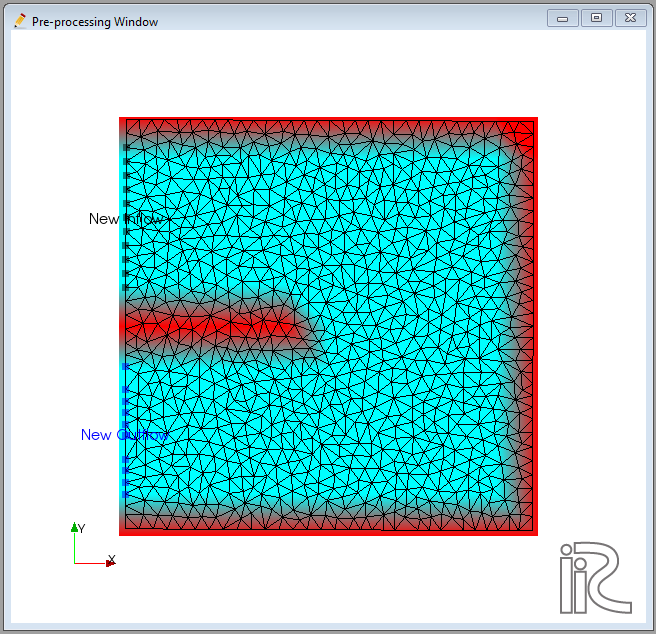
\includegraphics[height=3.5in]{OrdinaryBasin.png} 
   \caption{Aerial view of Ordinary Basin.   The red portion is elevation 4 meters, light blue is elevation 1 meters.  Inflow and outflow are shown.}
   \label{fig:OrdinaryBasin}
\end{figure}

\begin{figure}[h!] %  figure placement: here, top, bottom, or page
   \centering
   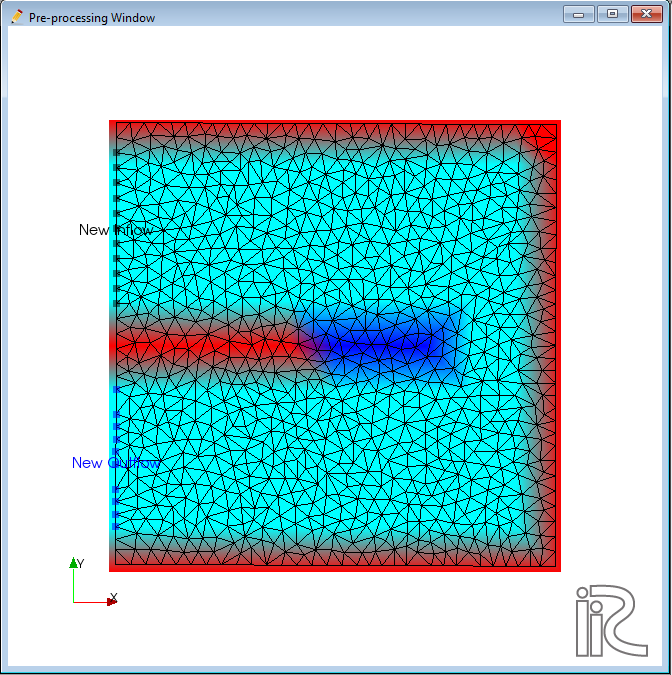
\includegraphics[height=3.5in]{BasinInBasin.png} 
   \caption{Aerial view of Basin-In-Basin concept.   The red portion is elevation 4 meters, light blue is elevation 1 meters, and the dark blue is 0 meters. Inflow and outflow are shown.}
   \label{fig:BasinInBasin}
\end{figure}

The dark blue ``hole'' is thought to confer advantage by reducing velocity of water in its vicinity, thus suspended constituents could conceivably be captured in this region, if indeed the velocity field is affected.  

\subsubsection*{Topographic Model for the Basins}
SToRM uses a topographic database in XYZ format.   Simple regular topographic files are built for the two basins \url{pond-no-hole.tpo} and \url{pond-in-pond.tpo}.

\section*{{Problem Statement}}
Build and run a SToRM model of the two conceptual designs described above using identical boundary conditions, write a brief report (like a lab report) and include:
\begin{enumerate}
\item Does there appear to be different circulation patterns in the two basins?
\item Produce vector and streamline plot of the flow pattern at in each model at large time (equilibrium); something like

\begin{figure}[h!] %  figure placement: here, top, bottom, or page
   \centering
   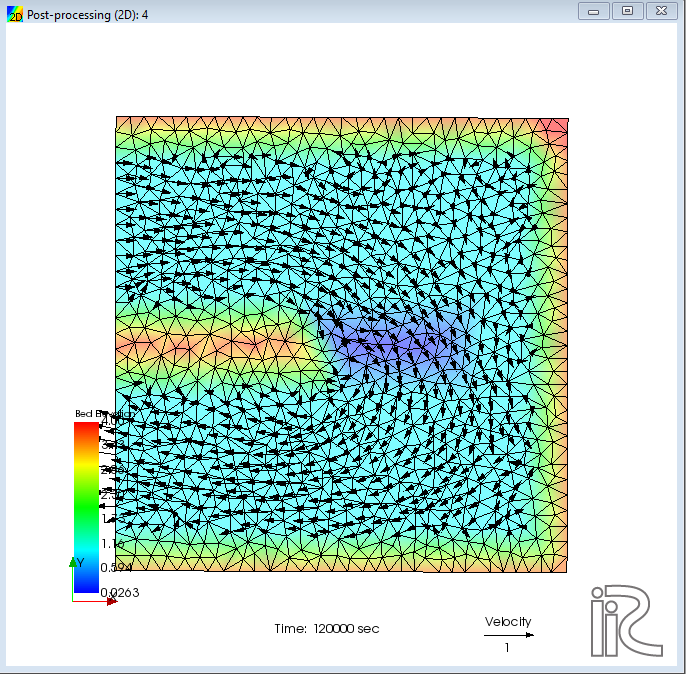
\includegraphics[height=3.5in]{TypicalVelocityField.png} 
   \caption{Basin-In-Basin concept, equilibrium plots for $Q_{in} = 2.0~cms$, $H_{out} = 2.0~m$.}
   \label{fig:TypicalVelocityField}
\end{figure}

\item Interpret the two sets of plots; is there influence of the hole; what is that influence; how would it affect water quality control if the goal is to remove suspended solids
\item (Advanced) Edit the \url{.tpo}, and move the hole to different locations; comment on any meaningful effects; Is the hole best placed as presented, or is closer to the inlet better; closer to the outlet?
\end{enumerate}

\begin{thebibliography}{}

\bibitem[USGS, 2011]{storm2011}
{USGS Geomorphology Laboratory} (2011).
\newblock System for Transport and River Modeling.   
\url{http://wwwbrr.cr.usgs.gov/projects/GEOMORPH_Lab/project-SToRM.html} Webpage last accessed, 12 Jan 2012.

\bibitem[McDonald and others, 2012]{mdswms2012}
{McDonald, R.R., Nelson, J.M., and Bennett, J.P.}, (2012).  
\textsl{in press}. Multi-dimensional surface-water modeling system user's guide: U.S. Geological Survey Techniques and Methods, 6-B2, 136 p.

%\bibitem[Google Earth, 2011]{GoogleEarth2011}
%{Google Earth, Google Inc.}, (2011). 
%\url{http://www.google.com/earth/index.html} 
%1600 Amphitheatre Parkway Mountain View, CA, 94043
%%
%\bibitem[Golden Software, 2010]{surfer2010}
%{Golden Software, Inc.}, (2010). Surfer 10.
%809 14th Street, Golden, Colorado 80401-1866, U.S.A.
%Phone: 303-279-1021 Fax: 303-279-0909
%\url{www.GoldenSoftware.com}

%\bibitem[Dixon, J. 2011]{dixon2011}
%{Dixon, J.}, (2011). 
%A Relation Between Select Hydraulic Properties and Sediment
%Transport Volume Through Experimental Culvert Configurations
%and Techniques for Measuring Sediment Transport Volumes.
%MS Thesis, Department of Civil and Environmental Engineering, Texas Tech University, 117 p.

\end{thebibliography}

\end{document}